\documentclass{article}
\usepackage{graphicx} % Required for inserting images
\usepackage[utf8]{inputenc}
\usepackage{polski}

\title{Przewidywanie ceny mieszkań na podstawie danych dostępnych na serwisie OTODOM}
\author{Jakub Stępkowski\\Politechnika Wrocławska }
\date{Czerwiec 2024}

\begin{document}

\maketitle

\section{Wstęp}
\section{Pozyskanie zbioru danych}
opisz scraper
\section{Przetwarzanie wstępne}
Zbiór danych zawiera następujące cechy:
\begin{enumerate}
    \item title - tytuł ogłoszenia
    \item address - adres mieszkania
    \item price - cena mieszkania
    \item rooms - liczba pokoi
    \item area - powierzchnia w $m^2$
    \item floor - piętro na którym znajduje się mieszkanie
    \item max\_floor - liczba pięter w budynku
    \item rent - wysokość renty
    \item energy\_certificate - 
    \item form\_of\_the\_property
    \item finishing\_condition
    \item balcony\_garden\_terrace
    \item parking\_place
    \item heating
    \item market
    \item advertisement\_type
    \item year\_of\_construction
    \item type\_of\_development
    \item finishing\_condition
    \item windows
    \item is\_elevator
\end{enumerate}
... dopisz opisy

Z adresu została wykorzystania wyłącznie nazwa osiedla, na którym znajduje się mieszkanie. Umieszczono ją w kolumnie \textit{adress\_estate}.
Cały zbiór zawiera 9843 mieszkań, jednak nie wszystkie oferty mają uzupełnione wszystkie cechy. Poniższy wykres pokazuje, dla każdej cechy, w ilu próbkach jest ona pusta:

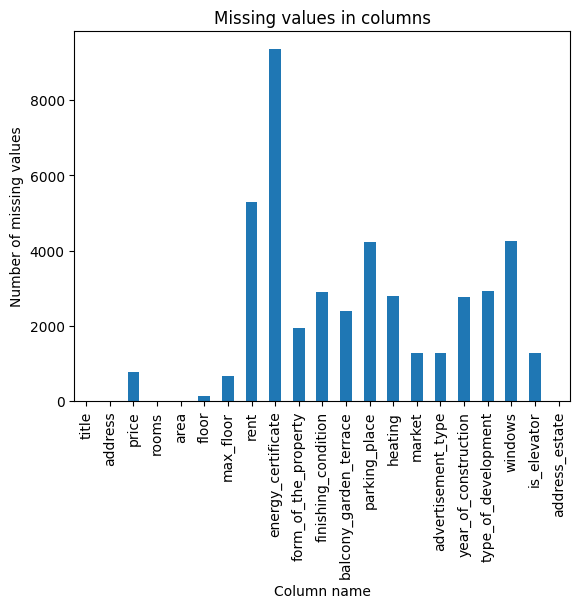
\includegraphics[width=.9\textwidth]{plots/missing_values.png}

Po analizie brakujących danych postanowiono wykorzystać następujące cechy:
rooms, area, address\_estate, floor, max\_floor, market, year\_of\_construction, finishing\_condition, is\_elevator.
Wszystkie oferty, które nie zawierały jakiejś z tych cech, zostały usunięte. W ten sposób zbiór danych został zredukowany do 4571 elementów. 

[ewentualnie opisz 10+ itd ale mowil ze go nie interesuje oczyszcanie xzbioru wiec pomijam]

Zbiór zawiera następujące cechy kategorialne: adress\_estate, market, finishing\_condition, is\_elevator. Cechy binarne (market i is\_elevator) zakodowano przez jedną cechę liczbową, gdzie 0 oznacza jedną z klas a 1 drugą. Cechy zawierające więcej kategorii (finishing\_condition i is\_elevator) zakodowano wykorzystując one hot encoding.

Wyizolowano cechę price jako cel predykcji. Ze względu na stabilność modeli postanowniono przewidywać cenę za metr kwadratowy, zamiast całkowitej ceny mieszkania.

Zbiór został podzielony na 3 podzbiory - treningowy, walidacyjny i testowy

Tak przygotowany zbiór danych przeskalowano z wykorzystaniem standardowego skalera, dopasowanego do zbioru treningowego (zarówno dla cech wejściowych jak i dla celu).



\section{Eksploracja danych}
wykresy

\section{Wybór i trening modeli}

\subsection{Model liniowy}

\subsection{Uogólniony  model liniowy}

\subsection{Sieć neuronowa}
Architektura wybranej sieci składała się z następujących warstw:
\begin{enumerate}
    \item Warstwa wejściowa - 11 neuronów
    \item Warstwa ukryta 1 - 256 neuronów z funkcją aktywacji ReLU
    \item Warstwa ukryta 2 - 128 neuronów z funkcją aktywacji ReLU
    \item Warstwa wyjściowa - 1 neuron
\end{enumerate}
Zastosowano gęste połączenia między kolejnymi warstwami. Została użyta funkcja aktywacji ReLU ze względu na jej niski koszt obliczeniowy. Po każdej z warstw ukrytych, na czas treningu, zastosowano dropout wielkości 30\% każdy w celu uniknięcia nadmiernego dopasowania do zbioru treningowego.

\textit{trening}

Do treningu został użyty algorytm optymalizacji Adam ze współczynnikiem uczenia 0.001. Pętla ucząca została wykonana 100 razy. Za każdym powtórzeniem odbywała się optymalizacja współczynników sieci na podstawie całego zbioru danych, pogrupowanego w serie po 16 próbek, w celu przyspieszenia obliczeń i lepszemu uogólnianiu. Wykorzystana funkcja straty to błąd średniokwadratowy.

Do implementacji sieci został wykorzystany moduł PyTorch.



\section{Porównanie modeli}

\section{Wnioski}

\end{document}
